\documentclass[twocolumn]{article}

\usepackage[utf8]{inputenc}
\usepackage{graphicx}
\usepackage{amssymb}
\usepackage{amsmath}
\providecommand{\brak}[1]{\ensuremath{\left(#1\right)}}

\title{Assignment 1}
\author{Gollapudi Sasank CS21BTECH11019}

\begin{document}

\maketitle
\section*{ Question 6 (a) :}
\noindent Using properties of proportion , solve for $x$. Given $x$ is positive :
\begin{align}
\frac{2x+\sqrt{4x^2-1}}{2x-\sqrt{4x^2-1}} &= 4 
\end{align}
\section*{Solution:}
From the properties of proportion
\begin{align}
     \frac{a}{b}  &=  \frac{c}{d} 
     \Rightarrow 
     \frac{a+b}{a-b} &= \frac{c+d}{c-d}
     \end{align}
The Given Equation is :
    \begin{align}
        \frac{2x+\sqrt{4x^2-1}}{2x-\sqrt{4x^2-1}} &= \frac {4}{1}
        \end{align}
    From (2) 
    \begin{align}
      \frac {2x+\sqrt{4x^2-1}+2x-\sqrt{4x^2-1}}{2x+\sqrt{4x^2-1}-2x+\sqrt{4x^2-1}} &= \frac {4+1}{4-1} \\ \Rightarrow
        \frac{4x}{2\sqrt{4x^2-1}} &= \frac {5}{3} \\   \Rightarrow
        \frac{6x}{5} &= \sqrt{4x^2-1} \\  \Rightarrow
        \frac{36x^2}{25} &= 4x^2-1 \\   \Rightarrow
         1 &= \brak {4 - \frac{36}{25}}x^2 \\   \Rightarrow
        x^2 &=\frac{25}{64} \\   \Rightarrow
        x &= \pm\frac{5}{8} 
    \end{align}
But Given $x$ is positive 
\begin{align}
   \Rightarrow x &= \frac{5}{8}  
   \end{align}
\section*{Verification with Graph:} 
If we draw the graph of 
y = f(x) = $\frac{2x+\sqrt{4x^2-1}}{2x-\sqrt{4x^2-1}}$
 and find point of intersection with $y$ = 4 ,\\ we get $x$ = 0.625 = $\frac{5}{8}$ \\    
\begin{figure}[h]  
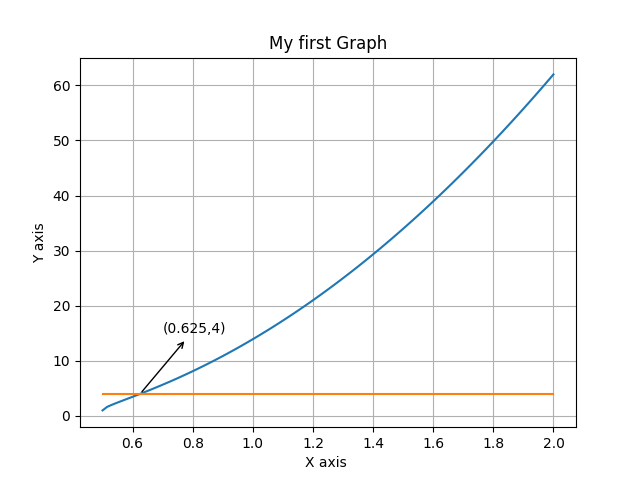
\includegraphics[width=\columnwidth]{output.png}
\caption{graph of y = f(x)}
\end{figure}
$\therefore x = \frac{5}{8} = 0.625 $
\end{document}
